%\begin{figure}[h]
%    \centering
%    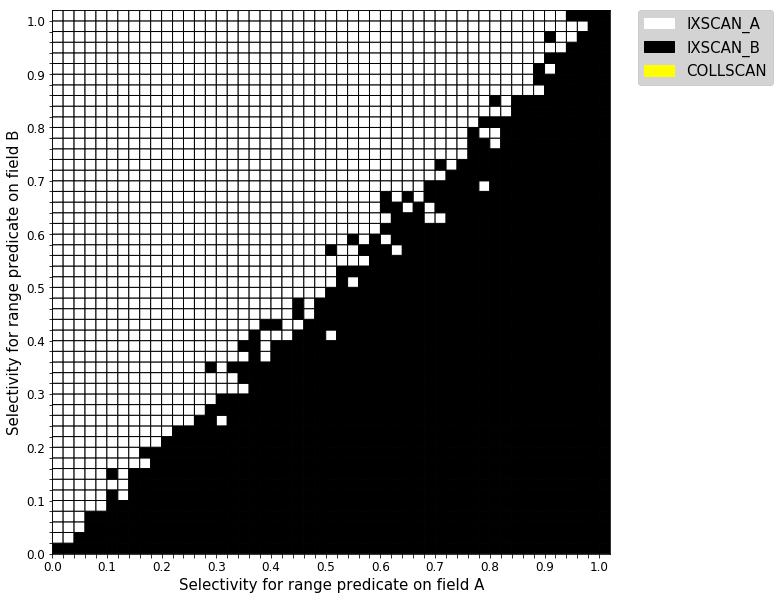
\includegraphics[width=\linewidth]{images/body/uniform_dist_practical_3095_10-23-2019_11_33_35.png}
%    \caption{Chosen query plan with both attributes indexed: MongoDB  never chooses a collection scan.}
%    \label{figure:v1-no-collscan}
%\end{figure}
%
%\begin{figure}[h]
%  \centering
%  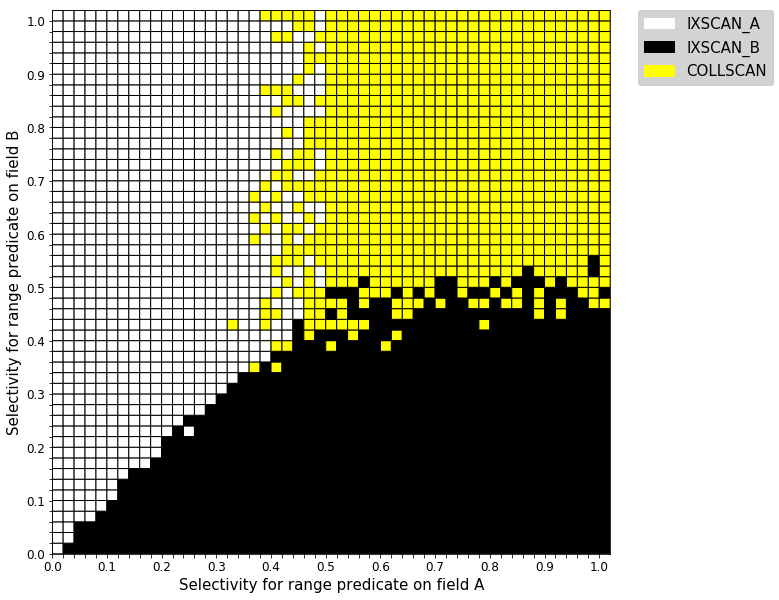
\includegraphics[width=\linewidth]{images/body/gird_sample_1.png}
%  \caption{Visual mapping of execution plans for different selectivities}
%  \label{figure:bothindex-optimalchoice}
%  \Description{\relname}
%\end{figure}

\section{Evaluation of MongoDB's \approachName Query Optimizer}
\label{sec:evaluation}

\begin{comment} Michael: done
\af{The textual values for accuracy, impact, maximum impact etc, seem to be the same as in VLDB 2021 submission! Please get the values from the latest experiments, and put them in.}
\end{comment}

In the following, we use our visualization approach from Section~\ref{sec:methodology} to assess the effectiveness of \approachName query optimization in MongoDB, in which we see which plans are chosen and which plans would actually be the best. We use varying physical designs for the data (varying sets of indexes).

%We quantify the impact of the performance bias issue and present the results through a heatmap. Through experiments we determine the accuracy of the query optimizer is only 69.29\%. Besides that, the optimal query plan is up to 86.83\% faster than MongoDB's choice. We demonstrate that the overall performance of the MongoDB query optimizer can be improved by 10.96\% if MongoDB adopt the optimal query plans. We then examine various database designs by repeating the experiment on different dataset with various kinds of distribution to further explore the impact of this issue. We find that the distribution of the dataset does not  influence MongoDB's query plan decisions. 



%\subsection{MongoDB Fails to Choose Collection Scans}
\subsection{Querying Indexed Collections}
\label{sec:evaluation_bothindexed}
In our first experiment, we investigate the case of conjunctive filter queries on two attributes where both of the queried attributes are indexed. The physical data design is, as described in Section~\ref{sec:methodology}, a collection with two integer-valued fields (A and B). In this experiment, each field has a uniform data distribution and each field has an index. Therefore, there are three reasonable query execution plans. One is to retrieve the documents that match the predicate on A, using the index on A, and then examine each to see whether the document also meets the predicate on B; this plan is called IXSCAN\_A, an index scan on A. We can symmetrically do an index scan on B using the index on B (IXSCAN\_B). Instead, we can perform a full collection scan, examining each document to see whether it meets the conjunction of both predicates (COLLSCAN). %Therefore, the balanced occurrences of IXSCAN\_A and IXSCAN\_B can be explained by the symmetrical design of the database. 

%We repeat the experiment with the modified version of MongoDB which takes the collection scan into the consideration. Nevertheless, the results remain unchanged, which confirms that MongoDB query optimizer has underlying issues when it evaluates query plans. For convenience,we name the original MongoDB and the modified version  V1 and V2, respectively.

Figure~\ref{fig:mongo-bothindexed-choices} plots the execution plans picked in this case by the \relname query optimizer. We observe that both IXSCAN\_A  and IXSCAN\_B are picked by the optimizer with equal chance, and as expected, the field where the query selectivity is lower (that is, fewer documents satisfy this predicate), has the index used.  This phenomenon suggests that the \approachName approach is capable of making efficient choices between index scans. The boundary between the two index scans is clear, and it forms a diagonal across the grid, which demonstrates that the query optimizer has a quite robust performance (the chosen plan does not usually change with small perturbations in the query). 

However, during all the runs of this experiment, we see that COLLSCAN was never the chosen plan. To see that this is surprising, we present the diagram showing which plan is actually the best for queries in this physical design (in Figure~\ref{fig:mongo-bothindexed-optimal}, which is the same as Figure~\ref{fig:grid-sample}) and what the ratio is between the cost of running the chosen plan compared to the true best plan (Figure~\ref{fig:mongo-bothindexed-perfimpact}). 

%\textbf{[[Diagram update needed: Figure~\ref{fig:mongo-bothindexed-perfimpact} showing the performance impact on two index structure, on \relname unmodified)]]}

\begin{figure*}[t]
%\newlength\plotheight%
\setlength\plotheight{\heightof{\includegraphics[width=0.30\textwidth]{images/results-single-index/v\mdbver/comprehensive_mongo_choice.png}}}
    \centering
    \subfigure[Chosen query plan with only attribute B indexed: MongoDB still never chooses a collection scan.]{\includegraphics[height=\plotheight]{images/results-single-index/v\mdbver/comprehensive_mongo_choice.png}\label{fig:mongo-singleindex-choices}}
    \hfill
    \subfigure[Optimal query plans for different selectivities with only one index.]{\includegraphics[height=\plotheight]{images/results-single-index/v\mdbver/comprehensive_practical_winner.png}\label{fig:mongo-singleindex-optimal}}
    \hfill
    \subfigure[Performance impact of MongoDB's query plan choices.]{\includegraphics[height=\plotheight-1em]{images/results-single-index/v\mdbver/comprehensive_summary_accuracy.png}\label{fig:mongo-singleindex-perfimpact}}
    \vspace*{-0.75\baselineskip}
    \caption{Effectiveness of MongoDB's query optimizer with conjunctive filter queries and only one attribute indexed.}
    \label{fig:singleindex-evaluation}
\end{figure*}
\begin{figure*}[t]
%\newlength\plotheight%
\setlength\plotheight{\heightof{\includegraphics[width=0.29\textwidth]{images/results-with-covering-index/v\mdbver/comprehensive_mongo_choice.png}}}
    \centering
    \subfigure[Chosen query plan with all attributes indexed and covering index available too.]{\includegraphics[height=\plotheight]{images/results-with-covering-index/v\mdbver/comprehensive_mongo_choice.png}\label{fig:mongo-coveringindex-choices}}
    \hfill
    \subfigure[Optimal query plans for different selectivities with covering index available too.]{\includegraphics[height=\plotheight]{images/results-with-covering-index/v\mdbver/comprehensive_practical_winner.png}\label{fig:mongo-coveringindex-optimal}}
    \hfill
    \subfigure[Performance impact of MongoDB's sub-optimal plan choices.]{\includegraphics[height=\plotheight-1em]{images/results-with-covering-index/v\mdbver/comprehensive_summary_accuracy.png}\label{fig:mongo-coveringindex-perfimpact}}
    \vspace*{-0.75\baselineskip}
    \caption{Effectiveness of MongoDB's query optimizer with all queried attributes being indexed including a covering index.}
    \label{fig:coveringindex-evaluation}
\end{figure*}


As one would expect, the performance of an index scan is significantly worse than a collection scan for a query that has very high selectivity on both fields (that is, each predicate is satisfied by most of the documents). At the extreme, if the query retrieves all documents in the collection, an index scan would first retrieve index documents and then use those index information to locate and fetch all documents. In contrast, a collection scan does not have index-access overhead; it directly retrieves all documents without using any index. Therefore, the top right corner of the grid in Figure~\ref{fig:mongo-bothindexed-optimal} is yellow, as expected. Since MongoDB does not choose a collection scan, in this corner of Figure~\ref{fig:mongo-bothindexed-perfimpact}, we see strong red, indicating that the chosen query runs substantially slower than the best possible execution plan.

% Michael: exp1-4, orig, uniform both
In summary, MongoDB's \approachName query optimizer shows an overall accuracy of just shy of 34\%
%(accuracy=33.92)
in this scenario, so about two thirds of the time there would be a better plan than one of the chosen index scan plans. The average impact factor of all those optimizer decisions is 1.7 (on average, the chosen query plan is 70\% slower than the optimal plan), with some chosen plans more than three times slower than a collection scan.

%We perform a case study to investigate the reason why the query optimizer does not choose collection scans. To begin with, we focus on the case where the selectivity of range predicate A and B both equal to one. In this case, the query intends to retrieve all documents in the collection. We execute the query with \verb|explain(allPlanExecution)| method to inspect the query execution statistics.  We observe that COLLSCAN is neither in the \verb|rejectedPlans| nor in the \verb|winningPlan|. We find out that MongoDB V1 does not consider COLLSCAN as a candidate query plan for this case, while COLLSCAN is theoretically the optimal query plan. To verify this observation, we inspect all query plans in the experiment, it turns out COLLSCAN has never been examined by the query optimizer. In conclusion, we prove that the MongoDB V1 has a defect that it does not consider collection scan as a candidate plan through a visualization and a case study. 


\vspace*{-0.5\baselineskip}
\subsection{Single Index Scenario}
%Our previous experiment only covered the scenario in which field A and field B both have an index. 
In the next experiment, we investigate the behavior of MongoDB's query optimizer with a physical structure where there is an index for only one of the attributes (field B). Again, we have uniformly distributed values in each field.

%Table~\ref{tbl:case5-8} shows the physical designs used in this section.

%\begin{table}[h]
%\begin{tabular}{lllll}
%\toprule
%{\small Case} & {\small Distribution of A} & {\small Distribution o%f B} & {\small Index on A} & {\small Index on B} \\ 
%\midrule
%5    & Uniform           & Uniform           & False      & True       \\
%6    & Uniform           & Linear            & False      & True       \\
%7    & Uniform           & Normal            & False      & True       \\
%8    & Uniform           & Zipfian           & False      & True   \\
%bottomrule
%\end{tabular}
%\caption{The database design of case 5, 6, 7 and 8 }
%\label{tbl:case5-8}
%\end{table}

Figure~\ref{fig:mongo-singleindex-choices} plots the query plans chosen by \relname and Figure~\ref{fig:mongo-singleindex-optimal} shows the optimal query plans. Figure~\ref{fig:mongo-singleindex-perfimpact} shows the performance impact of the preference bias issue. 
%Assuming MongoDB V1: Figure~\ref{fig:mongo-singleindex-choices} indicates that the collection scan has chance  to be chosen after we adding it to the query plan candidates. 
 %Nevertheless, 
%With the visualization in Figure~\ref{fig:mongo-singleindex-perfimpact}, we should observe that collection scan only been chosen when the impactfactor reaches the upper bound. In other words, MongoDB only realizes a collection scan is better when the relative performance of an index scan becomes extremely inefficient. We will analysis the root causeof this phenomenon in Section~\ref{sec:rootcauseanalysis}. %OR: \ref{chap:irc} ???

% Michael: exp2-4, orig, uniform single
From Figures~\ref{fig:mongo-singleindex-choices} and \ref{fig:mongo-singleindex-optimal} we see that the collection scan is actually the best as long as more than about 20\% of records satisfy the range predicate on B; however, even in these situations MongoDB chooses to use the available index on B; again, it never does a collection scan. Thus, the optimizer's choice is even less accurate than in the previous scenario, with an overall accuracy of 19\%. %(19.0\%)

And these sub-optimal choices sometimes come with a huge cost. Near the boundary between optimal choices, the two have similar costs (and so there is not much impact from choosing the index scan); however, in cases where most documents satisfy the predicate on B, we find that the plan chosen by MongoDB (the index scan) can execute over 400\% slower than the best plan for that query. The average slowdown of MongoDB's choice compared to the best possible is 140\%.

%Figure \ref{fig:casec4}, \ref{fig:casec5} and \ref{fig:casec6}  visualize query plans selected by MongoDB V2, the optimal query plans, and impact factors in this scenario. The experiment results verified our observation in section \ref{sec: eti}. That is, \approachName has the advantage that it is insensitive to the distribution of data.

% \begin{figure}[h]
%     \centering
%     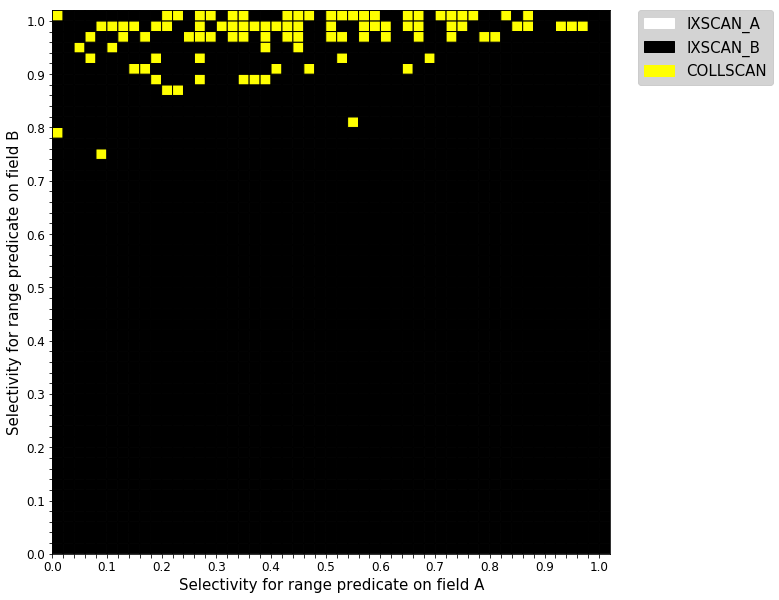
\includegraphics[width=0.4\linewidth]{images/body/uniform_dist_practical_5171_10-23-2019_11_41_32.png}
%     \caption{Visualization of query plans selected by MongoDB V2: case 5}
%     \label{fig:vs1}
% \end{figure}

% \begin{figure}[h]
%     \centering
%     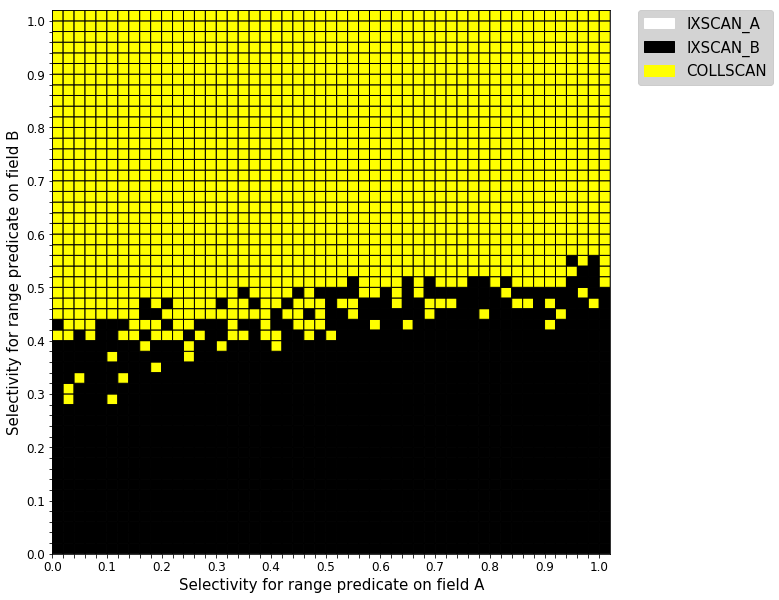
\includegraphics[width=0.4\linewidth]{images/body/uniform_dist_actual_5171_10-23-2019_11_41_32.png}
%     \caption{Visualization of the optimal query plans: case 5}
%     \label{fig:vs2}
% \end{figure}

%\begin{figure}[h]
%    \centering
%    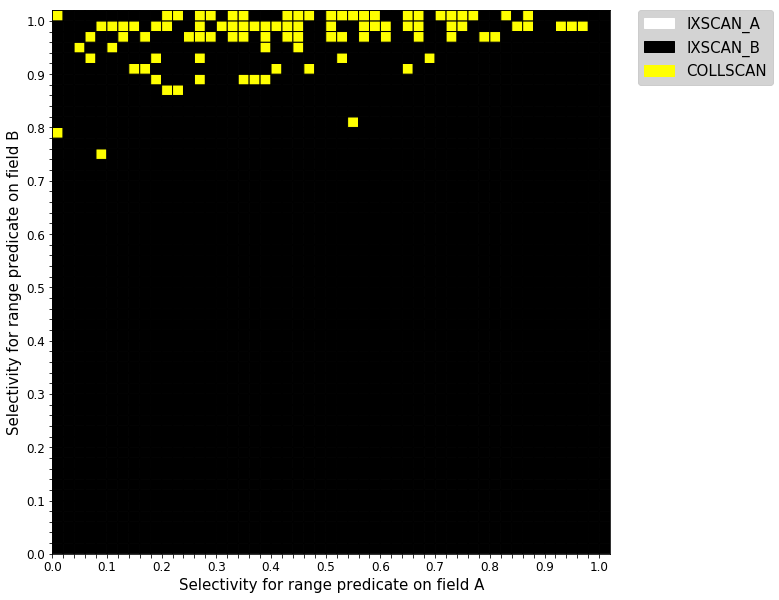
\includegraphics[width=0.7\linewidth]{images/body/uniform_dist_practical_5171_10-23-2019_11_41_32.png}
%    \caption{Visualization of query plans selected by MongoDB V2: case 5}
%    \label{fig:vs1}
%
%    \vspace{10pt}
%    \centering
%    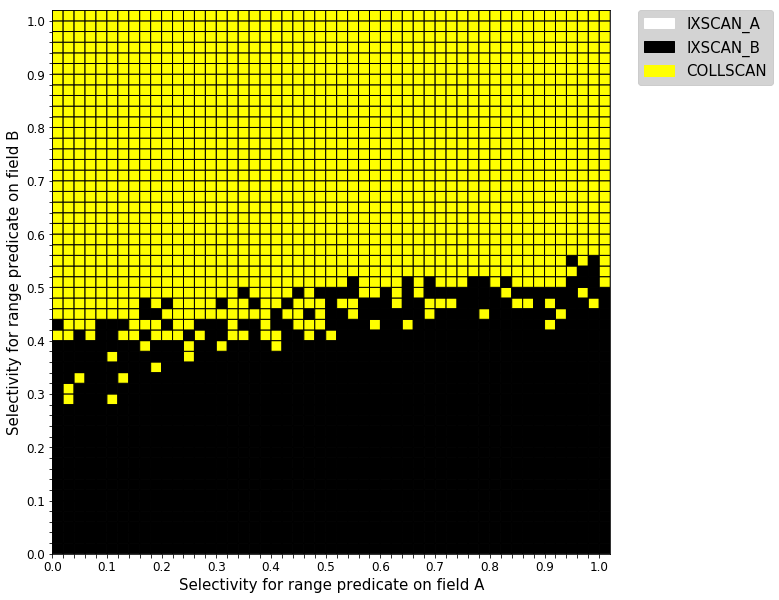
\includegraphics[width=0.7\linewidth]{images/body/uniform_dist_actual_5171_10-23-2019_11_41_32.png}
%    \caption{Visualization of the optimal query plans: case 5}
%    \label{fig:vs2}
%
%    \vspace{10pt}
%    \centering
%    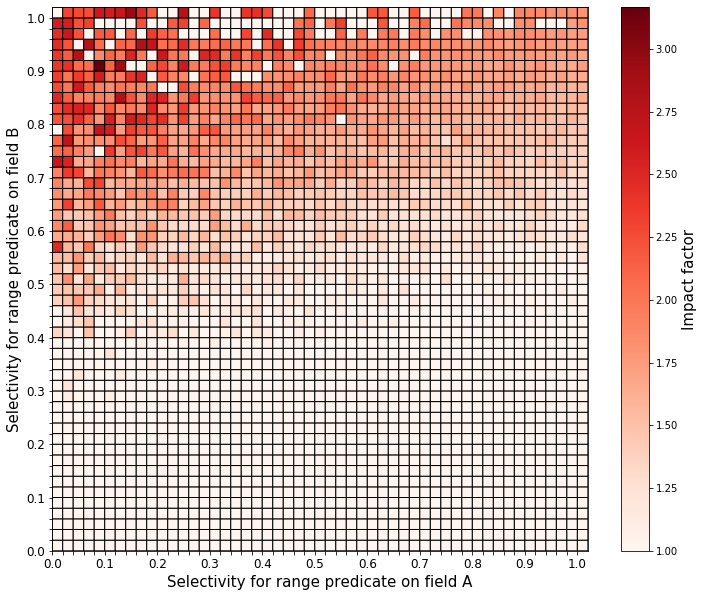
\includegraphics[width=0.65\linewidth]{images/body/uniform_dist_error_5171_11-09-2019_15_07_38.png}
%    \caption{Visualization of the impact factor: case 5}
%    \label{fig:vs3}
%\end{figure}

\vspace*{-0.5\baselineskip}
\subsection{Covering Index Scenario}
In our third experiment, we run our usual conjunctive queries over two attributes against a physical database design where, in addition to an index on each attribute, there is also a covering index on the combination (A,B) in that order. The power of the covering index is that query execution often does not need to access the document at all, as the information in the index is enough to determine whether or not the document matches both ranges in the predicate. 

Figure~\ref{fig:coveringindex-evaluation} shows the results of this third experiment. We again first visualize the query plans chosen by MongoDB's \approachName optimizer (Figure~\ref{fig:mongo-coveringindex-choices}), the middle plot shows the optimal plan (Figure~\ref{fig:mongo-coveringindex-optimal}), and the third plot is a visualization of the performance impact of MongoDB's suboptimal plan choices 
(Figure~\ref{fig:mongo-coveringindex-perfimpact}).

% Michael: exp1, comprehensive_summary_accuracy\=54.04_impact_factor\=1.19566.png
From the color distribution in Figure~\ref{fig:mongo-coveringindex-optimal}, we can see that an execution plan using the covering index would indeed be fastest in many cases and that the plan space where a full collection scan is best is now notably smaller than in the previous two scenarios. Furthermore, Figure~\ref{fig:mongo-coveringindex-choices} shows that MongoDB's \approachName optimizer indeed favors a covering index over a plan using an index just on A. But again we see that \approachName does not choose the collection scan even in cases where it is best, and also that it often chooses a plan that accesses through the index on B rather than the plan using the covering index. We see substantial inaccuracy and many cases where the performance is markedly worse than what the true optimal plan would deliver. Although the overall accuracy of \approachName is the best of the three scenarios with about 54\%, the average query speed is still slower than it could be, by 20\%.

\subsection{Performance with Varying Data Distributions}
Our experiments have so far always queried two numerical attributes with a uniform data distribution. We also did some extensive experiments with varying the data distributions of each attribute; for example, each field A and B could have uniform, normal, or zipfian distributions. However, we did not find any different behavior of MongoDB's query optimizer in these experiments from that shown so far for a uniform data distribution. The reason is probably that MongoDB chooses its best plan as soon as the first candidate plan produces the 100th result row, which is too early to show any significant difference between the varying data distributions. For space reasons, we omit the details of these runs from this paper and refer the interested reader to our forthcoming technical report. 

\paragraph{\textbf{Evaluation Summary.}} Overall, the experiments in this section demonstrate that while \approachName is a viable approach to query optimization with many good plan choices, it also suffers from a clear bias towards index scans over full collections scans. The question is whether this is simply an implementation bug specific to \relname, or whether it points to an inherit weakness of \approachName query optimization. We hence take a closer look into MongoDB's query optimizer in the next section.